% Options for packages loaded elsewhere
\PassOptionsToPackage{unicode}{hyperref}
\PassOptionsToPackage{hyphens}{url}
%
\documentclass[
]{book}
\usepackage{lmodern}
\usepackage{amsmath}
\usepackage{ifxetex,ifluatex}
\ifnum 0\ifxetex 1\fi\ifluatex 1\fi=0 % if pdftex
  \usepackage[T1]{fontenc}
  \usepackage[utf8]{inputenc}
  \usepackage{textcomp} % provide euro and other symbols
  \usepackage{amssymb}
\else % if luatex or xetex
  \usepackage{unicode-math}
  \defaultfontfeatures{Scale=MatchLowercase}
  \defaultfontfeatures[\rmfamily]{Ligatures=TeX,Scale=1}
\fi
% Use upquote if available, for straight quotes in verbatim environments
\IfFileExists{upquote.sty}{\usepackage{upquote}}{}
\IfFileExists{microtype.sty}{% use microtype if available
  \usepackage[]{microtype}
  \UseMicrotypeSet[protrusion]{basicmath} % disable protrusion for tt fonts
}{}
\makeatletter
\@ifundefined{KOMAClassName}{% if non-KOMA class
  \IfFileExists{parskip.sty}{%
    \usepackage{parskip}
  }{% else
    \setlength{\parindent}{0pt}
    \setlength{\parskip}{6pt plus 2pt minus 1pt}}
}{% if KOMA class
  \KOMAoptions{parskip=half}}
\makeatother
\usepackage{xcolor}
\IfFileExists{xurl.sty}{\usepackage{xurl}}{} % add URL line breaks if available
\IfFileExists{bookmark.sty}{\usepackage{bookmark}}{\usepackage{hyperref}}
\hypersetup{
  pdftitle={Data Exploration in R},
  pdfauthor={Prof.~Dr.~Jan Kirenz},
  hidelinks,
  pdfcreator={LaTeX via pandoc}}
\urlstyle{same} % disable monospaced font for URLs
\usepackage{color}
\usepackage{fancyvrb}
\newcommand{\VerbBar}{|}
\newcommand{\VERB}{\Verb[commandchars=\\\{\}]}
\DefineVerbatimEnvironment{Highlighting}{Verbatim}{commandchars=\\\{\}}
% Add ',fontsize=\small' for more characters per line
\usepackage{framed}
\definecolor{shadecolor}{RGB}{248,248,248}
\newenvironment{Shaded}{\begin{snugshade}}{\end{snugshade}}
\newcommand{\AlertTok}[1]{\textcolor[rgb]{0.94,0.16,0.16}{#1}}
\newcommand{\AnnotationTok}[1]{\textcolor[rgb]{0.56,0.35,0.01}{\textbf{\textit{#1}}}}
\newcommand{\AttributeTok}[1]{\textcolor[rgb]{0.77,0.63,0.00}{#1}}
\newcommand{\BaseNTok}[1]{\textcolor[rgb]{0.00,0.00,0.81}{#1}}
\newcommand{\BuiltInTok}[1]{#1}
\newcommand{\CharTok}[1]{\textcolor[rgb]{0.31,0.60,0.02}{#1}}
\newcommand{\CommentTok}[1]{\textcolor[rgb]{0.56,0.35,0.01}{\textit{#1}}}
\newcommand{\CommentVarTok}[1]{\textcolor[rgb]{0.56,0.35,0.01}{\textbf{\textit{#1}}}}
\newcommand{\ConstantTok}[1]{\textcolor[rgb]{0.00,0.00,0.00}{#1}}
\newcommand{\ControlFlowTok}[1]{\textcolor[rgb]{0.13,0.29,0.53}{\textbf{#1}}}
\newcommand{\DataTypeTok}[1]{\textcolor[rgb]{0.13,0.29,0.53}{#1}}
\newcommand{\DecValTok}[1]{\textcolor[rgb]{0.00,0.00,0.81}{#1}}
\newcommand{\DocumentationTok}[1]{\textcolor[rgb]{0.56,0.35,0.01}{\textbf{\textit{#1}}}}
\newcommand{\ErrorTok}[1]{\textcolor[rgb]{0.64,0.00,0.00}{\textbf{#1}}}
\newcommand{\ExtensionTok}[1]{#1}
\newcommand{\FloatTok}[1]{\textcolor[rgb]{0.00,0.00,0.81}{#1}}
\newcommand{\FunctionTok}[1]{\textcolor[rgb]{0.00,0.00,0.00}{#1}}
\newcommand{\ImportTok}[1]{#1}
\newcommand{\InformationTok}[1]{\textcolor[rgb]{0.56,0.35,0.01}{\textbf{\textit{#1}}}}
\newcommand{\KeywordTok}[1]{\textcolor[rgb]{0.13,0.29,0.53}{\textbf{#1}}}
\newcommand{\NormalTok}[1]{#1}
\newcommand{\OperatorTok}[1]{\textcolor[rgb]{0.81,0.36,0.00}{\textbf{#1}}}
\newcommand{\OtherTok}[1]{\textcolor[rgb]{0.56,0.35,0.01}{#1}}
\newcommand{\PreprocessorTok}[1]{\textcolor[rgb]{0.56,0.35,0.01}{\textit{#1}}}
\newcommand{\RegionMarkerTok}[1]{#1}
\newcommand{\SpecialCharTok}[1]{\textcolor[rgb]{0.00,0.00,0.00}{#1}}
\newcommand{\SpecialStringTok}[1]{\textcolor[rgb]{0.31,0.60,0.02}{#1}}
\newcommand{\StringTok}[1]{\textcolor[rgb]{0.31,0.60,0.02}{#1}}
\newcommand{\VariableTok}[1]{\textcolor[rgb]{0.00,0.00,0.00}{#1}}
\newcommand{\VerbatimStringTok}[1]{\textcolor[rgb]{0.31,0.60,0.02}{#1}}
\newcommand{\WarningTok}[1]{\textcolor[rgb]{0.56,0.35,0.01}{\textbf{\textit{#1}}}}
\usepackage{longtable,booktabs}
\usepackage{calc} % for calculating minipage widths
% Correct order of tables after \paragraph or \subparagraph
\usepackage{etoolbox}
\makeatletter
\patchcmd\longtable{\par}{\if@noskipsec\mbox{}\fi\par}{}{}
\makeatother
% Allow footnotes in longtable head/foot
\IfFileExists{footnotehyper.sty}{\usepackage{footnotehyper}}{\usepackage{footnote}}
\makesavenoteenv{longtable}
\usepackage{graphicx}
\makeatletter
\def\maxwidth{\ifdim\Gin@nat@width>\linewidth\linewidth\else\Gin@nat@width\fi}
\def\maxheight{\ifdim\Gin@nat@height>\textheight\textheight\else\Gin@nat@height\fi}
\makeatother
% Scale images if necessary, so that they will not overflow the page
% margins by default, and it is still possible to overwrite the defaults
% using explicit options in \includegraphics[width, height, ...]{}
\setkeys{Gin}{width=\maxwidth,height=\maxheight,keepaspectratio}
% Set default figure placement to htbp
\makeatletter
\def\fps@figure{htbp}
\makeatother
\setlength{\emergencystretch}{3em} % prevent overfull lines
\providecommand{\tightlist}{%
  \setlength{\itemsep}{0pt}\setlength{\parskip}{0pt}}
\setcounter{secnumdepth}{5}
\usepackage{booktabs}
\usepackage{amsmath}
\usepackage{booktabs}
\usepackage{caption}
\usepackage{longtable}
\ifluatex
  \usepackage{selnolig}  % disable illegal ligatures
\fi
\usepackage[]{natbib}
\bibliographystyle{apalike}

\title{Data Exploration in R}
\author{Prof.~Dr.~Jan Kirenz}
\date{2020-12-16}

\begin{document}
\maketitle

{
\setcounter{tocdepth}{1}
\tableofcontents
}
\hypertarget{welcome}{%
\chapter*{Welcome}\label{welcome}}
\addcontentsline{toc}{chapter}{Welcome}

This book provides an introduction to data exploration in R. To use the code in this book, activate the following packages:

\begin{Shaded}
\begin{Highlighting}[]
\FunctionTok{library}\NormalTok{(tidyverse)}
\FunctionTok{library}\NormalTok{(gt)}
\end{Highlighting}
\end{Shaded}

To illustrate the different data exploration methods, we use the dataset \texttt{wage} from \citet{James2000}, which contains wage and other data for a group of 3000 male workers in the Mid-Atlantic region.

\begin{Shaded}
\begin{Highlighting}[]
\FunctionTok{library}\NormalTok{(tidyverse)}

\NormalTok{wage\_df }\OtherTok{\textless{}{-}} \FunctionTok{read\_csv}\NormalTok{(}\StringTok{"https://raw.githubusercontent.com/kirenz/datasets/master/wage.csv"}\NormalTok{)}
\end{Highlighting}
\end{Shaded}

The data frame includes 3000 observations on the following 11 variables:

\begin{itemize}
\tightlist
\item
  \texttt{X1}: An ID variable
\item
  \texttt{year}: Year that wage information was recorded
\item
  \texttt{age}: Age of worker
\item
  \texttt{maritl}: A factor with levels: 1. Never Married 2. Married 3. Widowed 4. Divorced and 5. Separated indicating marital status
\item
  \texttt{race}: A factor with levels: 1. White 2. Black 3. Asian and 4. Other indicating race
\item
  \texttt{education}: A factor with levels: 1. \textless{} HS Grad 2. HS Grad 3. Some College 4. College Grad and 5. Advanced Degree indicating education level
\item
  \texttt{region}: Region of the country (mid-atlantic only)
\item
  \texttt{jobclass}: A factor with levels: 1. Industrial and 2. Information indicating type of job
\item
  \texttt{health}: A factor with levels: 1. \textless=Good and 2. \textgreater=Very Good indicating health level of worker
\item
  \texttt{health\_ins}: A factor with levels: 1. Yes and 2. No indicating whether worker has health insurance
\item
  \texttt{logwage}: Log of workers wage
\item
  \texttt{wage}: Workers raw wage
\end{itemize}

Note that this book mainly covers the use of a collection of R packages called the \href{https://www.tidyverse.org}{tidyverse}, an ecosystem of packages designed with common APIs and a shared philosophy. An R package is simply a bundle of functions, documentation, and data sets. There are about 25 packages in the tidyverse and they are especially designed for data science and share an underlying design philosophy, grammar, and data structures.

\begin{center}\rule{0.5\linewidth}{0.5pt}\end{center}

This online book is licensed using the \href{https://creativecommons.org/licenses/by-nc/2.0/}{Creative Commons Attribution-NonCommercial 2.0 Generic (CC BY-NC 2.0) License}.

\hfill\break

\hypertarget{tables}{%
\chapter{Counts and Tables}\label{tables}}

You should use this method if the data is:

\begin{itemize}
\tightlist
\item
  Categorical
\end{itemize}

In this chapter you will learn how to do data exploration for categorical variables using tables (also called contingency tables) and counts.

\hypertarget{counts}{%
\section{Counts}\label{counts}}

Count for one variable:

\begin{itemize}
\tightlist
\item
  Use data \texttt{wage\_df}.
\item
  Perform \href{https://dplyr.tidyverse.org/reference/count.html}{\texttt{count()}} on \texttt{maritl}
\item
  Sort the values.
\item
  Use \href{https://gt.rstudio.com}{\texttt{gt()}} to print the table.
\end{itemize}

\begin{Shaded}
\begin{Highlighting}[]
\NormalTok{wage\_df }\SpecialCharTok{\%\textgreater{}\%} 
  \FunctionTok{count}\NormalTok{(maritl,}
        \AttributeTok{sort =} \ConstantTok{TRUE}\NormalTok{) }\SpecialCharTok{\%\textgreater{}\%} 
  \FunctionTok{gt}\NormalTok{()}
\end{Highlighting}
\end{Shaded}

\captionsetup[table]{labelformat=empty,skip=1pt}
\begin{longtable}{lc}
\toprule
maritl & n \\ 
\midrule
2. Married & 2074 \\ 
1. Never Married & 648 \\ 
4. Divorced & 204 \\ 
5. Separated & 55 \\ 
3. Widowed & 19 \\ 
\bottomrule
\end{longtable}

Count two variables:

\begin{itemize}
\tightlist
\item
  Use data \texttt{wage\_df}.
\item
  Perform \href{https://dplyr.tidyverse.org/reference/count.html}{count()} on \texttt{maritl} and \texttt{education}
\item
  Sort the values.
\item
  Use \href{https://gt.rstudio.com}{gt()} to print the table.
\end{itemize}

\begin{Shaded}
\begin{Highlighting}[]
\NormalTok{wage\_df }\SpecialCharTok{\%\textgreater{}\%} 
  \FunctionTok{count}\NormalTok{(maritl, education,}
        \AttributeTok{sort=} \ConstantTok{TRUE}\NormalTok{) }\SpecialCharTok{\%\textgreater{}\%} 
  \FunctionTok{gt}\NormalTok{()}
\end{Highlighting}
\end{Shaded}

\captionsetup[table]{labelformat=empty,skip=1pt}
\begin{longtable}{llc}
\toprule
maritl & education & n \\ 
\midrule
2. Married & 2. HS Grad & 651 \\ 
2. Married & 4. College Grad & 487 \\ 
2. Married & 3. Some College & 421 \\ 
2. Married & 5. Advanced Degree & 341 \\ 
1. Never Married & 2. HS Grad & 219 \\ 
2. Married & 1. < HS Grad & 174 \\ 
1. Never Married & 3. Some College & 164 \\ 
1. Never Married & 4. College Grad & 143 \\ 
4. Divorced & 2. HS Grad & 73 \\ 
1. Never Married & 1. < HS Grad & 62 \\ 
1. Never Married & 5. Advanced Degree & 60 \\ 
4. Divorced & 3. Some College & 52 \\ 
4. Divorced & 4. College Grad & 41 \\ 
4. Divorced & 5. Advanced Degree & 22 \\ 
5. Separated & 2. HS Grad & 20 \\ 
4. Divorced & 1. < HS Grad & 16 \\ 
5. Separated & 1. < HS Grad & 14 \\ 
5. Separated & 3. Some College & 11 \\ 
5. Separated & 4. College Grad & 9 \\ 
3. Widowed & 2. HS Grad & 8 \\ 
3. Widowed & 4. College Grad & 5 \\ 
3. Widowed & 1. < HS Grad & 2 \\ 
3. Widowed & 3. Some College & 2 \\ 
3. Widowed & 5. Advanced Degree & 2 \\ 
5. Separated & 5. Advanced Degree & 1 \\ 
\bottomrule
\end{longtable}

Obtain the sum of a quantitative variable (\texttt{wage}) for different levels of a categorical variable (\texttt{maritl}) by using \texttt{wt\ =}:

\begin{Shaded}
\begin{Highlighting}[]
\NormalTok{wage\_df }\SpecialCharTok{\%\textgreater{}\%}  
  \FunctionTok{count}\NormalTok{(maritl,}
        \AttributeTok{wt =}\NormalTok{ wage,}
        \AttributeTok{name =} \StringTok{"Sum"}\NormalTok{) }\SpecialCharTok{\%\textgreater{}\%} 
  \FunctionTok{gt}\NormalTok{()}
\end{Highlighting}
\end{Shaded}

\captionsetup[table]{labelformat=empty,skip=1pt}
\begin{longtable}{lr}
\toprule
maritl & Sum \\ 
\midrule
1. Never Married & 60092.052 \\ 
2. Married & 246516.180 \\ 
3. Widowed & 1891.234 \\ 
4. Divorced & 21044.489 \\ 
5. Separated & 5566.868 \\ 
\bottomrule
\end{longtable}

\hypertarget{total-counts}{%
\section{Total counts}\label{total-counts}}

Total counts are an useful way to represent the observations that fall into each combination of the levels of categorical variables. We create a contingency table of the two categorical variables \texttt{jobclass} and \texttt{race} and call the result \texttt{tab}:

\begin{Shaded}
\begin{Highlighting}[]
\NormalTok{tab }\OtherTok{\textless{}{-}} \FunctionTok{table}\NormalTok{(wage\_df}\SpecialCharTok{$}\NormalTok{jobclass, wage\_df}\SpecialCharTok{$}\NormalTok{race)}
\NormalTok{tab}
\end{Highlighting}
\end{Shaded}

\begin{verbatim}
##                 
##                  1. White 2. Black 3. Asian 4. Other
##   1. Industrial      1325      111       86       22
##   2. Information     1155      182      104       15
\end{verbatim}

\hypertarget{joint-proportions}{%
\section{Joint proportions}\label{joint-proportions}}

We can also view the percentage of each cell in relation to the total amount of all observations (here n = 3000). Therefore, you have to simply divide the numbers from our total counts with 3.000.

The following code generates tables of \emph{joint} proportions:

\begin{Shaded}
\begin{Highlighting}[]
\CommentTok{\# joint proportions}
\FunctionTok{prop.table}\NormalTok{(tab) }
\end{Highlighting}
\end{Shaded}

\begin{verbatim}
##                 
##                     1. White    2. Black    3. Asian    4. Other
##   1. Industrial  0.441666667 0.037000000 0.028666667 0.007333333
##   2. Information 0.385000000 0.060666667 0.034666667 0.005000000
\end{verbatim}

For example, around 44\% of all people in the dataset are white industrial workers.

\hypertarget{conditional-proportions-columns}{%
\section{Conditional proportions: columns}\label{conditional-proportions-columns}}

You also may want to know the probability that workers have a certain jobclass, given that they have a particular ethnical background. This is a so called conditional probability. Conditional probability represents the chance that one event will occur given that a second event has already occurred.

The following code generates tables of \emph{conditional} proportions:

\begin{Shaded}
\begin{Highlighting}[]
\CommentTok{\# conditional on columns}
\FunctionTok{prop.table}\NormalTok{(tab, }\DecValTok{2}\NormalTok{)  }
\end{Highlighting}
\end{Shaded}

\begin{verbatim}
##                 
##                   1. White  2. Black  3. Asian  4. Other
##   1. Industrial  0.5342742 0.3788396 0.4526316 0.5945946
##   2. Information 0.4657258 0.6211604 0.5473684 0.4054054
\end{verbatim}

We performed a columnwise evaluation and are now able to answer the following question:

\begin{itemize}
\tightlist
\item
  Approximately what proportion of all white workers are industrial workers?
\item
  The answer is: around 53\%.
\end{itemize}

\hypertarget{conditional-proportions-rows}{%
\section{Conditional proportions: rows}\label{conditional-proportions-rows}}

Now we want to obtain the probability that workers have a certain race, given their jobclass.

\begin{Shaded}
\begin{Highlighting}[]
\CommentTok{\# conditional on rows}
\FunctionTok{prop.table}\NormalTok{(tab, }\DecValTok{1}\NormalTok{)  }
\end{Highlighting}
\end{Shaded}

\begin{verbatim}
##                 
##                    1. White   2. Black   3. Asian   4. Other
##   1. Industrial  0.85816062 0.07189119 0.05569948 0.01424870
##   2. Information 0.79326923 0.12500000 0.07142857 0.01030220
\end{verbatim}

We performed a rowwise evaluation and are now able to answer the following question:

\begin{itemize}
\tightlist
\item
  Approximately what proportion of all industrial workers are white?
\item
  The answer is: around 86\%.
\end{itemize}

\hypertarget{chi-squared-test-of-independence}{%
\section{Chi-squared Test of Independence}\label{chi-squared-test-of-independence}}

Finally, let's test the hypothesis whether the variable \texttt{jobclass} is independent of the variable \texttt{race} at .05 significance level.

\begin{Shaded}
\begin{Highlighting}[]
\FunctionTok{chisq.test}\NormalTok{(tab)  }
\end{Highlighting}
\end{Shaded}

\begin{verbatim}
## 
##  Pearson's Chi-squared test
## 
## data:  tab
## X-squared = 29.331, df = 3, p-value = 1.908e-06
\end{verbatim}

As the p-value is smaller than the .05 significance level, we reject the null hypothesis that the jobclass is independent of the race of the workers.

\hypertarget{heatmap}{%
\chapter{Heatmap}\label{heatmap}}

You should use this method if the data is:

\begin{itemize}
\tightlist
\item
  Categorical
\end{itemize}

In this chapter you will learn how to do some simple data explorations for categorical variables using heatmaps with the function \href{https://ggplot2.tidyverse.org/reference/geom_bin2d.html}{geom\_bin2d()}

Basic plot:

\begin{Shaded}
\begin{Highlighting}[]
\NormalTok{wage\_df }\SpecialCharTok{\%\textgreater{}\%}
  \FunctionTok{ggplot}\NormalTok{(}\FunctionTok{aes}\NormalTok{(jobclass, education)) }\SpecialCharTok{+}
  \FunctionTok{geom\_bin2d}\NormalTok{() }\SpecialCharTok{+}
  \FunctionTok{scale\_fill\_gradient}\NormalTok{(}\AttributeTok{low =} \StringTok{"gray85"}\NormalTok{, }\AttributeTok{high =} \StringTok{"steelblue"}\NormalTok{) }
\end{Highlighting}
\end{Shaded}

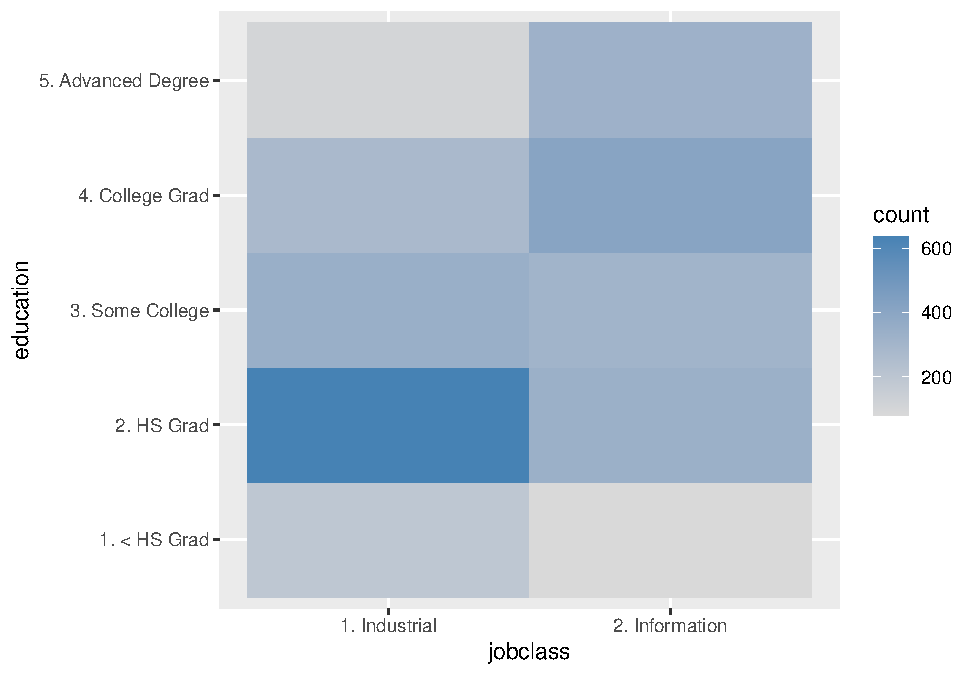
\includegraphics{exploration_files/figure-latex/heat-1.pdf}

Plot with some adjustments:

\begin{Shaded}
\begin{Highlighting}[]
\NormalTok{wage\_df }\SpecialCharTok{\%\textgreater{}\%}
  \FunctionTok{ggplot}\NormalTok{(}\FunctionTok{aes}\NormalTok{(jobclass, education)) }\SpecialCharTok{+}
  \FunctionTok{geom\_bin2d}\NormalTok{(}\AttributeTok{binwidth =} \FunctionTok{c}\NormalTok{(}\DecValTok{1}\NormalTok{, }\DecValTok{1}\NormalTok{), }\AttributeTok{alpha =} \FloatTok{0.8}\NormalTok{) }\SpecialCharTok{+}
  \FunctionTok{theme\_classic}\NormalTok{() }\SpecialCharTok{+} 
  \FunctionTok{scale\_fill\_gradient}\NormalTok{(}\AttributeTok{low =} \StringTok{"gray85"}\NormalTok{, }\AttributeTok{high =} \StringTok{"steelblue"}\NormalTok{) }\SpecialCharTok{+}
  \FunctionTok{labs}\NormalTok{(}\AttributeTok{fill =} \StringTok{"number of }\SpecialCharTok{\textbackslash{}n}\StringTok{ workers"}\NormalTok{, }\AttributeTok{y =} \StringTok{"Education"}\NormalTok{, }\AttributeTok{x =} \StringTok{"Job class"}\NormalTok{)}
\end{Highlighting}
\end{Shaded}

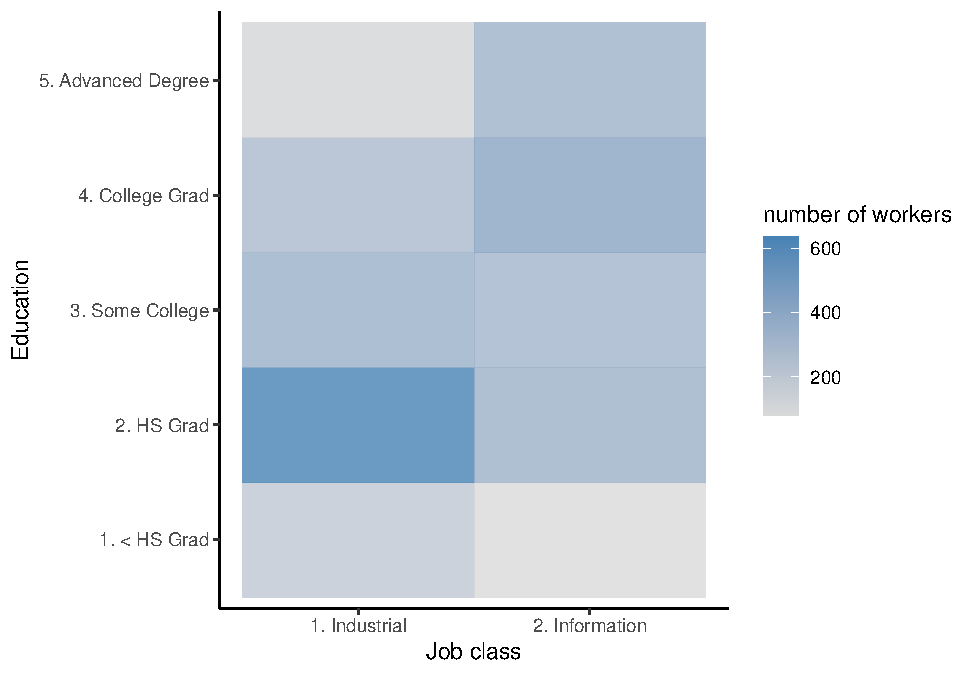
\includegraphics{exploration_files/figure-latex/heat-2-1.pdf}

\hypertarget{barplot}{%
\chapter{Barplot}\label{barplot}}

You should use this method if the data is:

\begin{itemize}
\tightlist
\item
  Categorical
\end{itemize}

In this chapter you will learn how to do some simple data explorations for categorical variables using barplots.

\hypertarget{one-variable}{%
\section{One variable}\label{one-variable}}

\begin{Shaded}
\begin{Highlighting}[]
\NormalTok{wage\_df }\SpecialCharTok{\%\textgreater{}\%} 
  \FunctionTok{ggplot}\NormalTok{(}\FunctionTok{aes}\NormalTok{(}\AttributeTok{x =}\NormalTok{ maritl)) }\SpecialCharTok{+}
  \FunctionTok{geom\_bar}\NormalTok{()}
\end{Highlighting}
\end{Shaded}

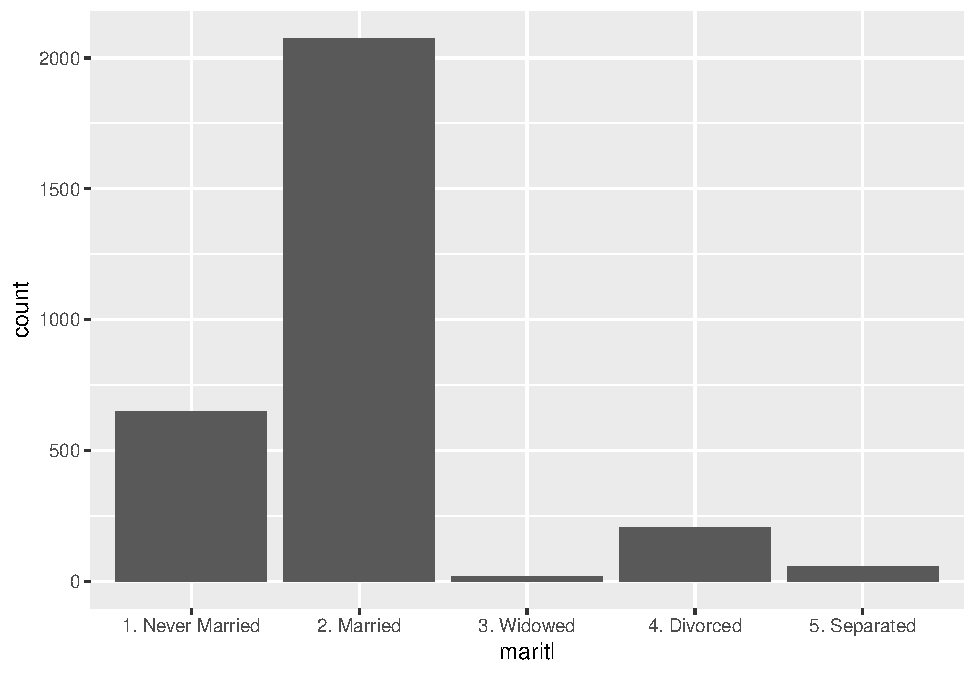
\includegraphics{exploration_files/figure-latex/bar-1-1.pdf}

\hypertarget{two-variables}{%
\section{Two variables}\label{two-variables}}

\hypertarget{stacked-barplot}{%
\subsection{Stacked barplot}\label{stacked-barplot}}

Absolute values:

\begin{Shaded}
\begin{Highlighting}[]
\NormalTok{wage\_df }\SpecialCharTok{\%\textgreater{}\%} 
  \FunctionTok{ggplot}\NormalTok{(}\FunctionTok{aes}\NormalTok{(}\AttributeTok{x =}\NormalTok{ maritl, }\AttributeTok{fill =}\NormalTok{ education)) }\SpecialCharTok{+} 
  \FunctionTok{geom\_bar}\NormalTok{()}
\end{Highlighting}
\end{Shaded}

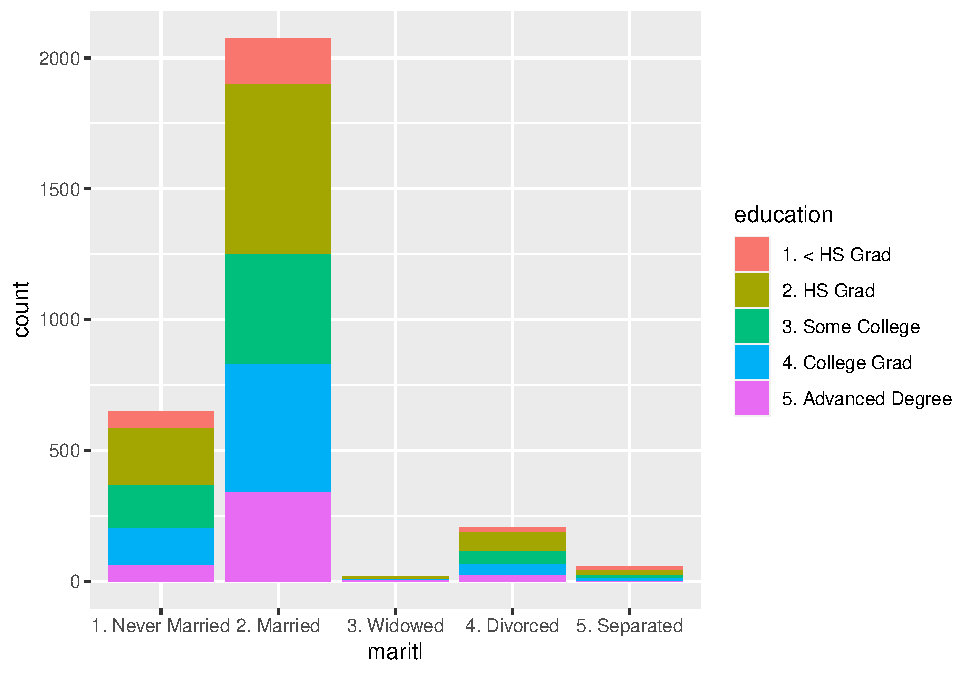
\includegraphics{exploration_files/figure-latex/bar-stacked-1.pdf}

Relative values:

\begin{Shaded}
\begin{Highlighting}[]
\NormalTok{wage\_df }\SpecialCharTok{\%\textgreater{}\%} 
  \FunctionTok{ggplot}\NormalTok{(}\FunctionTok{aes}\NormalTok{(}\AttributeTok{x =}\NormalTok{ maritl, }\AttributeTok{fill =}\NormalTok{ education)) }\SpecialCharTok{+}
  \FunctionTok{geom\_bar}\NormalTok{(}\AttributeTok{position =} \StringTok{"fill"}\NormalTok{) }\SpecialCharTok{+}
  \FunctionTok{ggtitle}\NormalTok{(}\StringTok{"Marital Status"}\NormalTok{, }\StringTok{"Overview"}\NormalTok{) }\SpecialCharTok{+}
  \FunctionTok{xlab}\NormalTok{(}\StringTok{" Marital Status"}\NormalTok{) }\SpecialCharTok{+}
  \FunctionTok{ylab}\NormalTok{(}\StringTok{"Number of People"}\NormalTok{) }\SpecialCharTok{+}
  \FunctionTok{theme\_classic}\NormalTok{() }\SpecialCharTok{+}
  \FunctionTok{scale\_fill\_brewer}\NormalTok{(}\AttributeTok{palette =} \StringTok{"Blues"}\NormalTok{) }\SpecialCharTok{+}
  \FunctionTok{theme}\NormalTok{(}\AttributeTok{legend.title =} \FunctionTok{element\_blank}\NormalTok{())}
\end{Highlighting}
\end{Shaded}

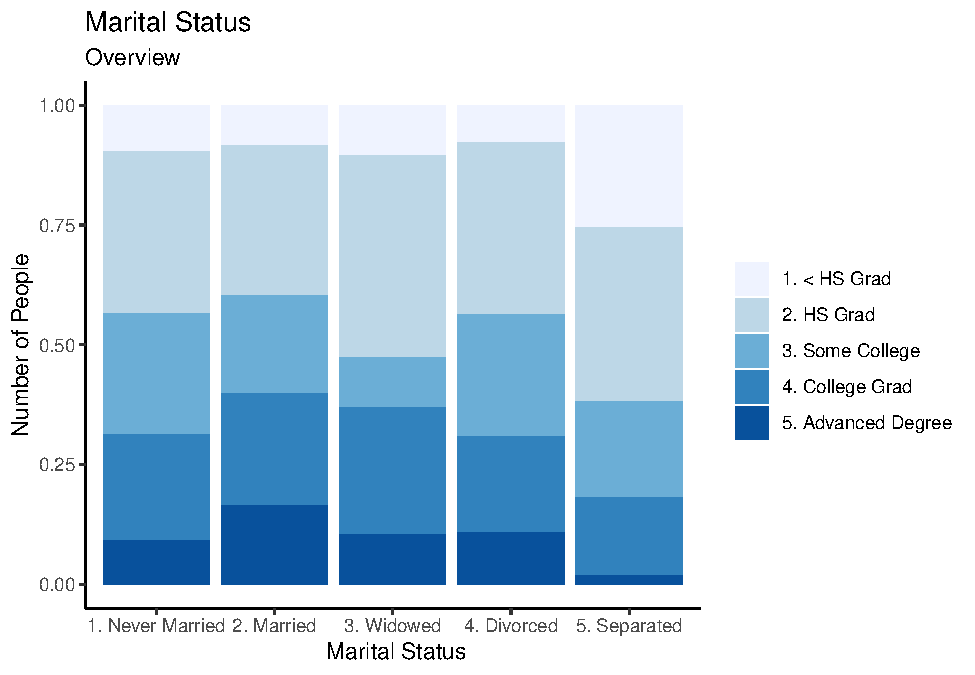
\includegraphics{exploration_files/figure-latex/bar-stacked-rel-1.pdf}

\hypertarget{side-by-side-barplot}{%
\subsection{Side-by-side barplot}\label{side-by-side-barplot}}

Basic plot:

\begin{Shaded}
\begin{Highlighting}[]
\NormalTok{wage\_df }\SpecialCharTok{\%\textgreater{}\%} 
  \FunctionTok{ggplot}\NormalTok{(}\FunctionTok{aes}\NormalTok{(}\AttributeTok{x =}\NormalTok{ maritl, }\AttributeTok{fill =}\NormalTok{ education)) }\SpecialCharTok{+}
  \FunctionTok{geom\_bar}\NormalTok{(}\AttributeTok{position =} \StringTok{"dodge"}\NormalTok{) }
\end{Highlighting}
\end{Shaded}

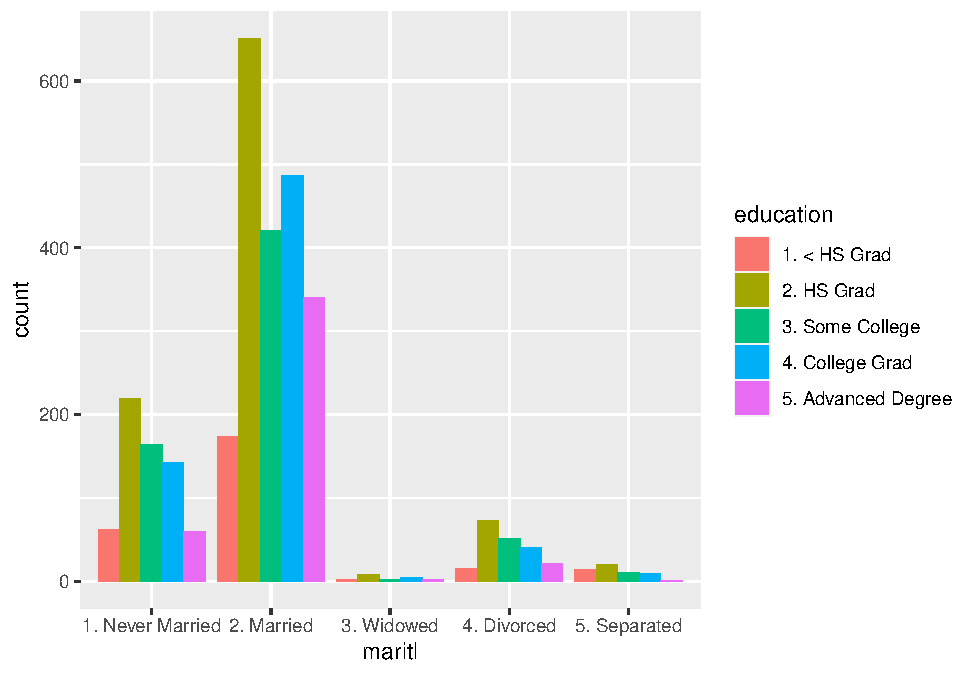
\includegraphics{exploration_files/figure-latex/bar-side-1.pdf}

Plot with some adjustments:

\begin{Shaded}
\begin{Highlighting}[]
\NormalTok{wage\_df }\SpecialCharTok{\%\textgreater{}\%} 
  \FunctionTok{ggplot}\NormalTok{(}\FunctionTok{aes}\NormalTok{(}\AttributeTok{x =}\NormalTok{ maritl, }\AttributeTok{fill =}\NormalTok{ education)) }\SpecialCharTok{+}
  \FunctionTok{geom\_bar}\NormalTok{(}\AttributeTok{position =} \StringTok{"dodge"}\NormalTok{) }\SpecialCharTok{+}
  \FunctionTok{ggtitle}\NormalTok{(}\StringTok{"Marital Status"}\NormalTok{, }\StringTok{"Overview"}\NormalTok{) }\SpecialCharTok{+}
  \FunctionTok{xlab}\NormalTok{(}\StringTok{" Marital Status"}\NormalTok{) }\SpecialCharTok{+}
  \FunctionTok{ylab}\NormalTok{(}\StringTok{"Number of People"}\NormalTok{) }\SpecialCharTok{+}
  \FunctionTok{theme\_classic}\NormalTok{() }\SpecialCharTok{+}
  \FunctionTok{scale\_fill\_brewer}\NormalTok{(}\AttributeTok{palette =} \StringTok{"Blues"}\NormalTok{) }\SpecialCharTok{+}
  \FunctionTok{theme}\NormalTok{(}\AttributeTok{legend.title =} \FunctionTok{element\_blank}\NormalTok{())}
\end{Highlighting}
\end{Shaded}

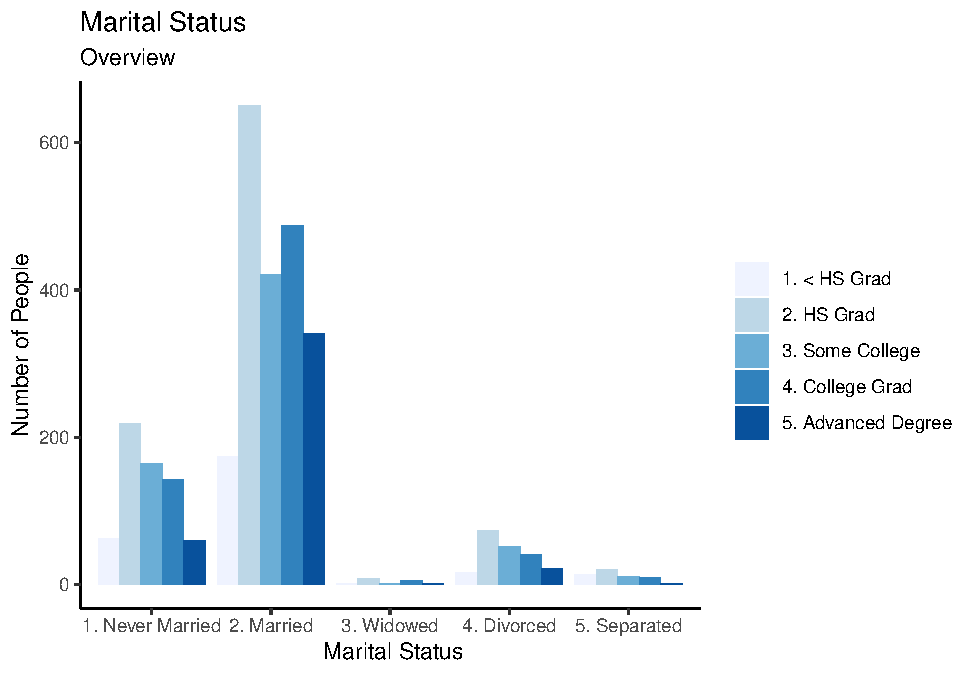
\includegraphics{exploration_files/figure-latex/bar-side-adj-1.pdf}

\hypertarget{faceted-barplot}{%
\subsection{Faceted barplot}\label{faceted-barplot}}

Basic plot:

\begin{Shaded}
\begin{Highlighting}[]
\NormalTok{wage\_df }\SpecialCharTok{\%\textgreater{}\%} 
  \FunctionTok{ggplot}\NormalTok{(}\FunctionTok{aes}\NormalTok{(}\AttributeTok{x =}\NormalTok{ maritl)) }\SpecialCharTok{+}
  \FunctionTok{geom\_bar}\NormalTok{(}\AttributeTok{position =} \StringTok{"dodge"}\NormalTok{) }\SpecialCharTok{+}
  \FunctionTok{facet\_wrap}\NormalTok{(}\SpecialCharTok{\textasciitilde{}}\NormalTok{ education)}
\end{Highlighting}
\end{Shaded}

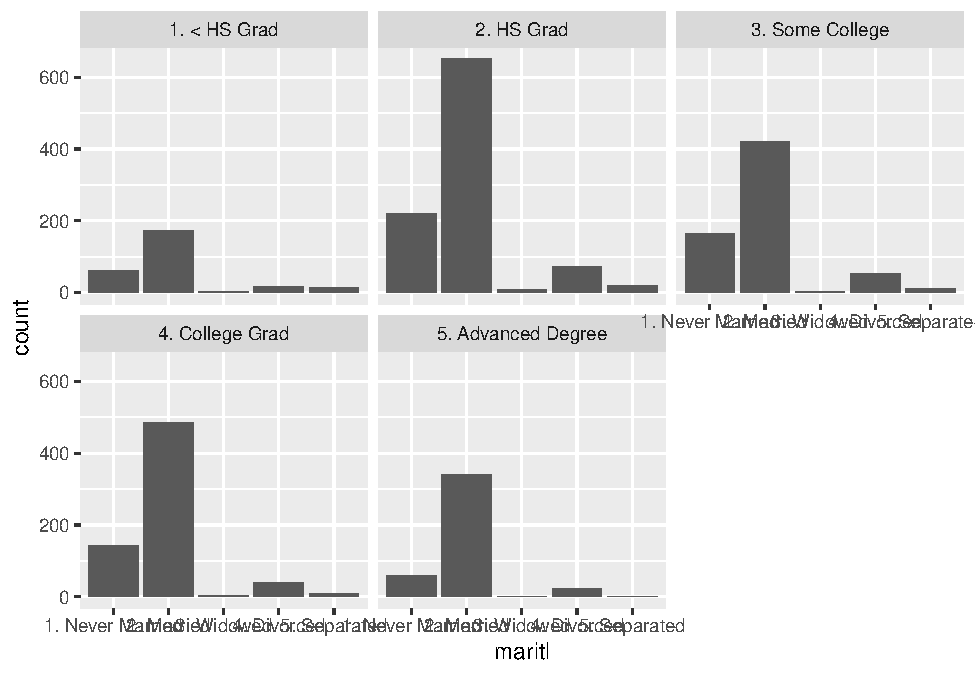
\includegraphics{exploration_files/figure-latex/bar-facet-1.pdf}

Plot with some adjustments to change our x labels using \href{https://ggplot2.tidyverse.org/articles/ggplot2-specs.html}{justifications}):

Horizontal and vertical justification have the same parameterisation, either a string (``top'', ``middle'', ``bottom'', ``left'', ``center'', ``right'') or a number between 0 and 1:"

\begin{itemize}
\tightlist
\item
  top = 1, middle = 0.5, bottom = 0
\item
  left = 0, center = 0.5, right = 1
\end{itemize}

\begin{Shaded}
\begin{Highlighting}[]
\NormalTok{wage\_df }\SpecialCharTok{\%\textgreater{}\%} 
  \FunctionTok{ggplot}\NormalTok{(}\FunctionTok{aes}\NormalTok{(}\AttributeTok{x =}\NormalTok{ maritl)) }\SpecialCharTok{+}
  \FunctionTok{geom\_bar}\NormalTok{(}\AttributeTok{position =} \StringTok{"dodge"}\NormalTok{) }\SpecialCharTok{+}
  \FunctionTok{facet\_wrap}\NormalTok{(}\SpecialCharTok{\textasciitilde{}}\NormalTok{ education) }\SpecialCharTok{+} 
  \FunctionTok{ggtitle}\NormalTok{(}\StringTok{"Marital Status"}\NormalTok{, }\StringTok{"Overview"}\NormalTok{) }\SpecialCharTok{+}
  \FunctionTok{xlab}\NormalTok{(}\StringTok{" Marital Status"}\NormalTok{) }\SpecialCharTok{+}
  \FunctionTok{ylab}\NormalTok{(}\StringTok{"Number of People"}\NormalTok{) }\SpecialCharTok{+}
  \FunctionTok{theme\_classic}\NormalTok{() }\SpecialCharTok{+}
  \FunctionTok{theme}\NormalTok{(}\AttributeTok{legend.title =} \FunctionTok{element\_blank}\NormalTok{()) }\SpecialCharTok{+}
  \FunctionTok{theme}\NormalTok{(}\AttributeTok{axis.text.x =} \FunctionTok{element\_text}\NormalTok{(}\AttributeTok{angle =} \DecValTok{90}\NormalTok{, }
                                   \AttributeTok{vjust =} \FloatTok{0.5}\NormalTok{, }
                                   \AttributeTok{hjust=}  \DecValTok{1}\NormalTok{))}
\end{Highlighting}
\end{Shaded}

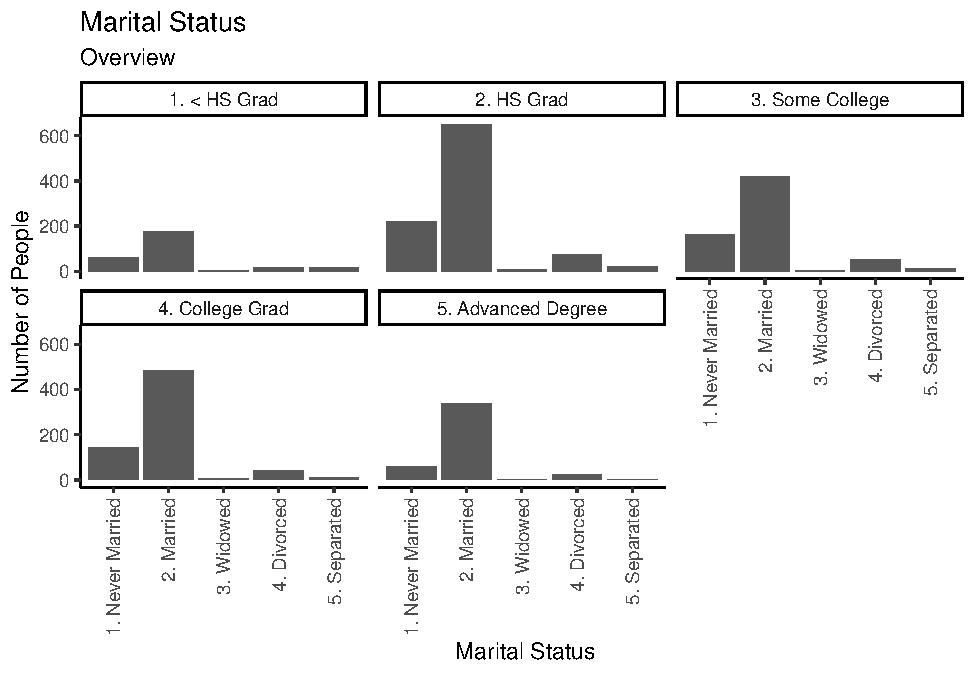
\includegraphics{exploration_files/figure-latex/bar-favet-adj-1.pdf}

\hypertarget{histogram}{%
\chapter{Histogram}\label{histogram}}

You should use this method if the data is:

\begin{itemize}
\tightlist
\item
  Numeric
\end{itemize}

\hypertarget{one-variable-1}{%
\section{One variable}\label{one-variable-1}}

\hypertarget{basic-histogram}{%
\subsection{Basic Histogram}\label{basic-histogram}}

Basic plot:

\begin{Shaded}
\begin{Highlighting}[]
\NormalTok{wage\_df }\SpecialCharTok{\%\textgreater{}\%} 
  \FunctionTok{ggplot}\NormalTok{(}\FunctionTok{aes}\NormalTok{(}\AttributeTok{x =}\NormalTok{ wage)) }\SpecialCharTok{+}
  \FunctionTok{geom\_histogram}\NormalTok{()}
\end{Highlighting}
\end{Shaded}

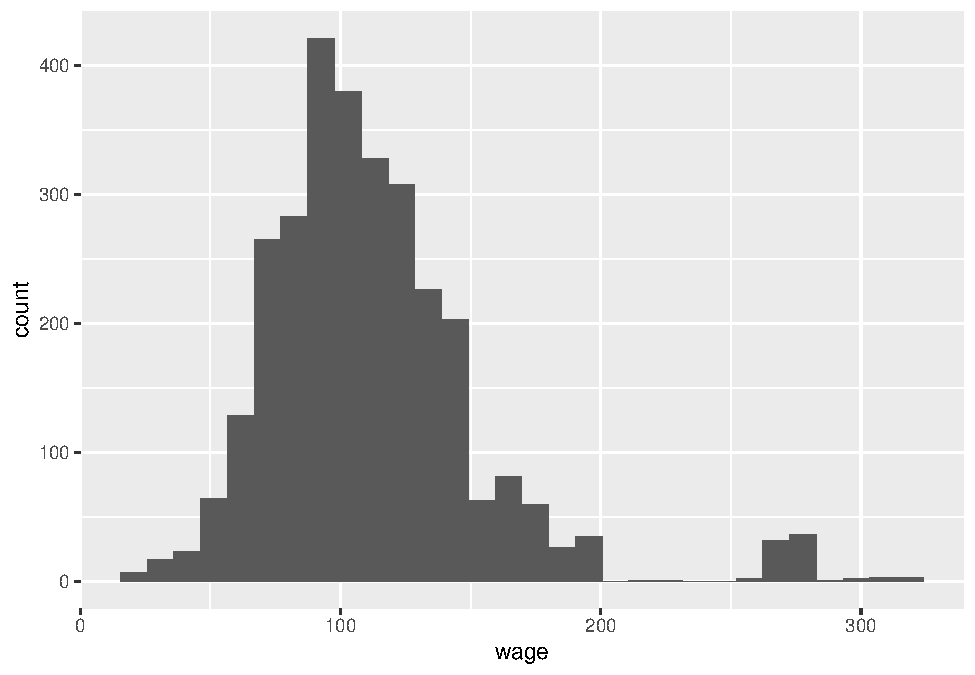
\includegraphics{exploration_files/figure-latex/hist-1-1.pdf}

\hypertarget{bins}{%
\subsection{Bins}\label{bins}}

Adjust number of bins:

\begin{Shaded}
\begin{Highlighting}[]
\NormalTok{wage\_df }\SpecialCharTok{\%\textgreater{}\%} 
  \FunctionTok{ggplot}\NormalTok{(}\FunctionTok{aes}\NormalTok{(}\AttributeTok{x =}\NormalTok{ wage)) }\SpecialCharTok{+}
  \FunctionTok{geom\_histogram}\NormalTok{(}\AttributeTok{bins =} \DecValTok{20}\NormalTok{)}
\end{Highlighting}
\end{Shaded}

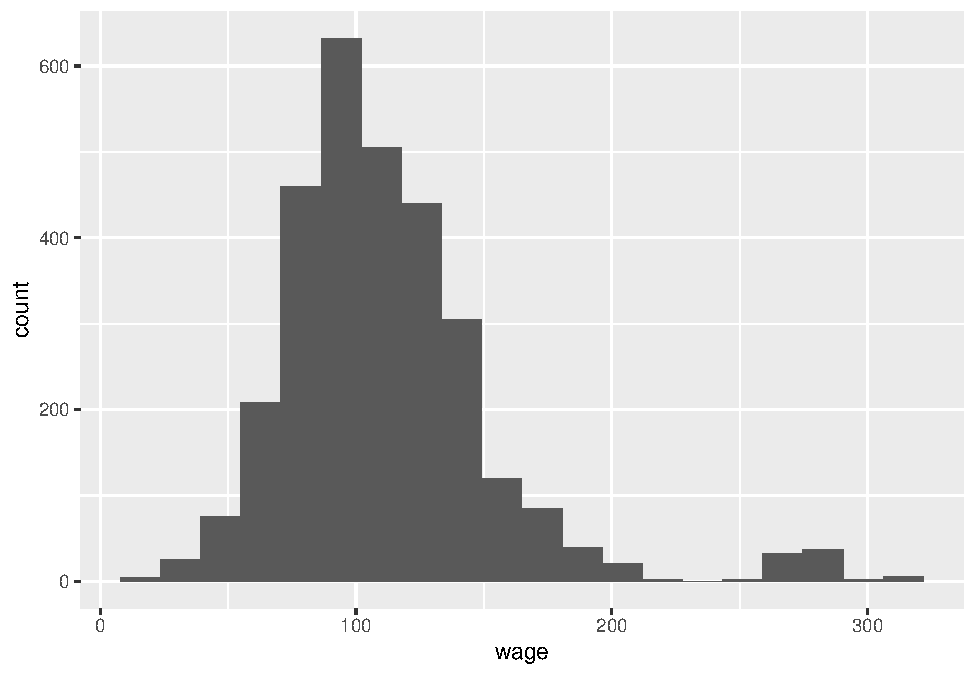
\includegraphics{exploration_files/figure-latex/hist-bins-1.pdf}

\hypertarget{binwidth}{%
\subsection{Binwidth}\label{binwidth}}

Instead of using bins, you can also change the binwidth:

\begin{Shaded}
\begin{Highlighting}[]
\NormalTok{wage\_df }\SpecialCharTok{\%\textgreater{}\%} 
  \FunctionTok{ggplot}\NormalTok{(}\FunctionTok{aes}\NormalTok{(}\AttributeTok{x =}\NormalTok{ wage)) }\SpecialCharTok{+}
  \FunctionTok{geom\_histogram}\NormalTok{(}\AttributeTok{binwidth =} \DecValTok{10}\NormalTok{)}
\end{Highlighting}
\end{Shaded}

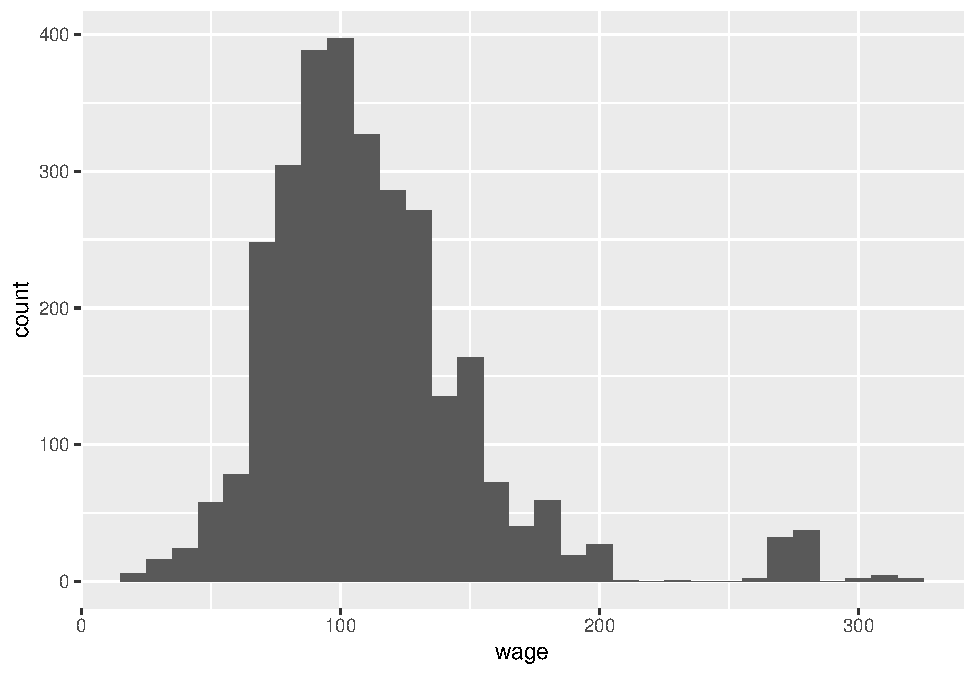
\includegraphics{exploration_files/figure-latex/hist-binwidth-1.pdf}

\hypertarget{two-variables-1}{%
\section{Two variables}\label{two-variables-1}}

\hypertarget{faceted-histogram}{%
\subsection{Faceted histogram}\label{faceted-histogram}}

\begin{Shaded}
\begin{Highlighting}[]
\NormalTok{wage\_df }\SpecialCharTok{\%\textgreater{}\%} 
  \FunctionTok{ggplot}\NormalTok{(}\FunctionTok{aes}\NormalTok{(}\AttributeTok{x =}\NormalTok{ wage)) }\SpecialCharTok{+}
  \FunctionTok{geom\_histogram}\NormalTok{() }\SpecialCharTok{+}
  \FunctionTok{facet\_wrap}\NormalTok{( }\SpecialCharTok{\textasciitilde{}}\NormalTok{ education)}
\end{Highlighting}
\end{Shaded}

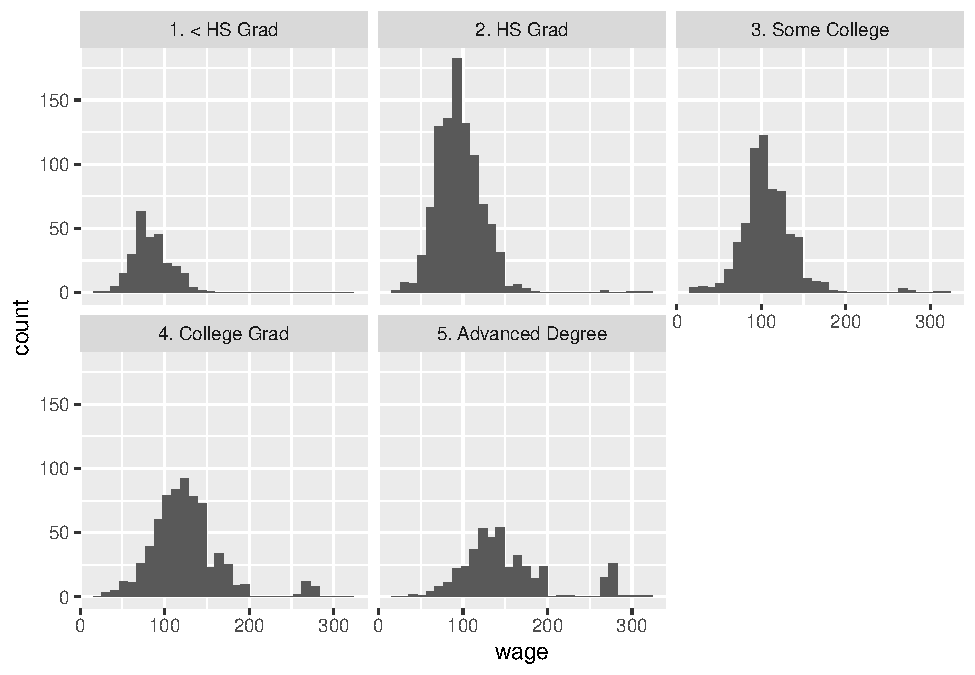
\includegraphics{exploration_files/figure-latex/hist-facet-1.pdf}

\hypertarget{stacked-histogram}{%
\subsection{Stacked histogram}\label{stacked-histogram}}

\begin{Shaded}
\begin{Highlighting}[]
\NormalTok{wage\_df }\SpecialCharTok{\%\textgreater{}\%} 
  \FunctionTok{ggplot}\NormalTok{(}\FunctionTok{aes}\NormalTok{(}\AttributeTok{x =}\NormalTok{ wage, }\AttributeTok{fill =}\NormalTok{ education)) }\SpecialCharTok{+}
  \FunctionTok{geom\_histogram}\NormalTok{(}\AttributeTok{alpha =} \FloatTok{0.4}\NormalTok{)}
\end{Highlighting}
\end{Shaded}

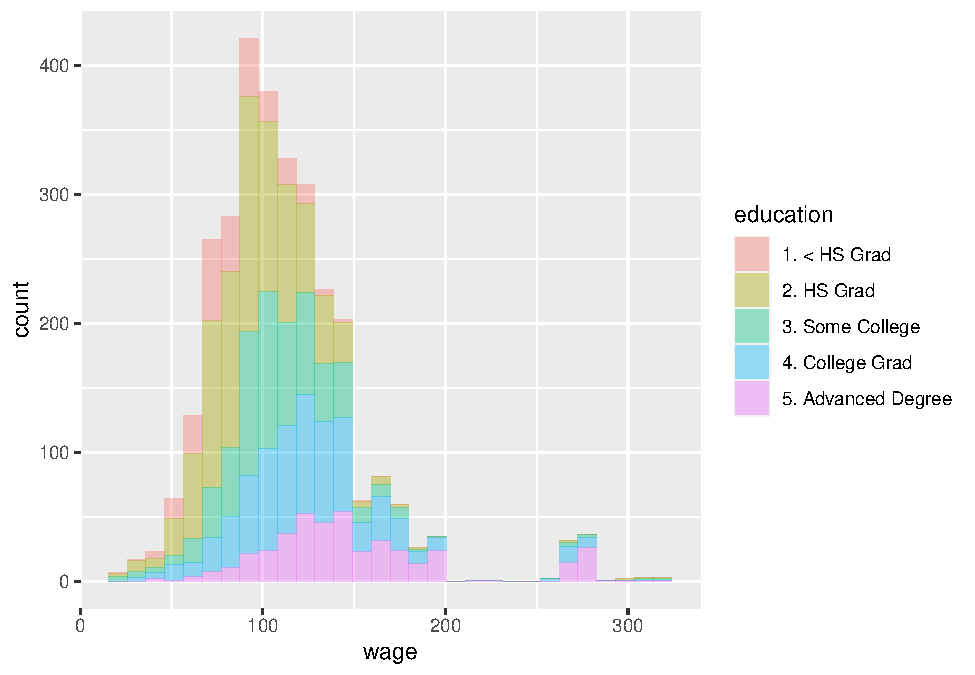
\includegraphics{exploration_files/figure-latex/hist-stacked-1.pdf}

\hypertarget{density}{%
\chapter{Density plots}\label{density}}

You should use this method if the data is:

\begin{itemize}
\tightlist
\item
  Numeric and continuous
\end{itemize}

In this chapter you will learn how to do some simple data explorations for numerical variables using density plots.

\hypertarget{one-variable-2}{%
\section{One variable}\label{one-variable-2}}

\begin{Shaded}
\begin{Highlighting}[]
\NormalTok{wage\_df }\SpecialCharTok{\%\textgreater{}\%} 
  \FunctionTok{ggplot}\NormalTok{(}\FunctionTok{aes}\NormalTok{(}\AttributeTok{x =}\NormalTok{ wage)) }\SpecialCharTok{+}
  \FunctionTok{geom\_density}\NormalTok{()}
\end{Highlighting}
\end{Shaded}

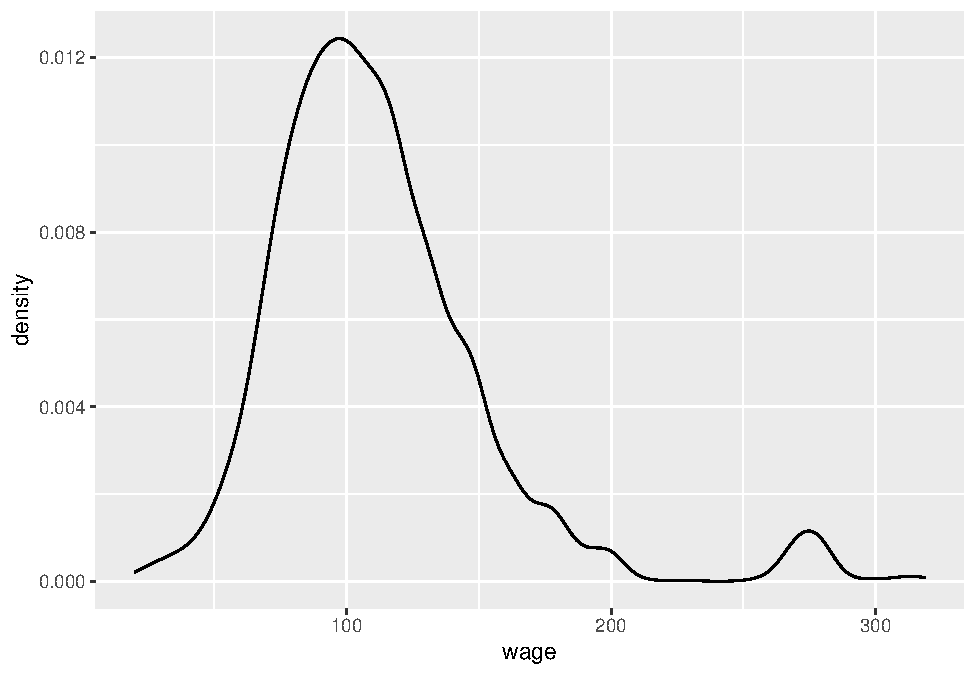
\includegraphics{exploration_files/figure-latex/unnamed-chunk-3-1.pdf}

\hypertarget{two-variables-2}{%
\section{Two variables}\label{two-variables-2}}

Combine your numeric variable with a categorical variable:

\begin{Shaded}
\begin{Highlighting}[]
\NormalTok{wage\_df }\SpecialCharTok{\%\textgreater{}\%} 
  \FunctionTok{ggplot}\NormalTok{(}\FunctionTok{aes}\NormalTok{(}\AttributeTok{x =}\NormalTok{ wage, }\AttributeTok{fill =}\NormalTok{ education)) }\SpecialCharTok{+} 
  \FunctionTok{geom\_density}\NormalTok{() }
\end{Highlighting}
\end{Shaded}

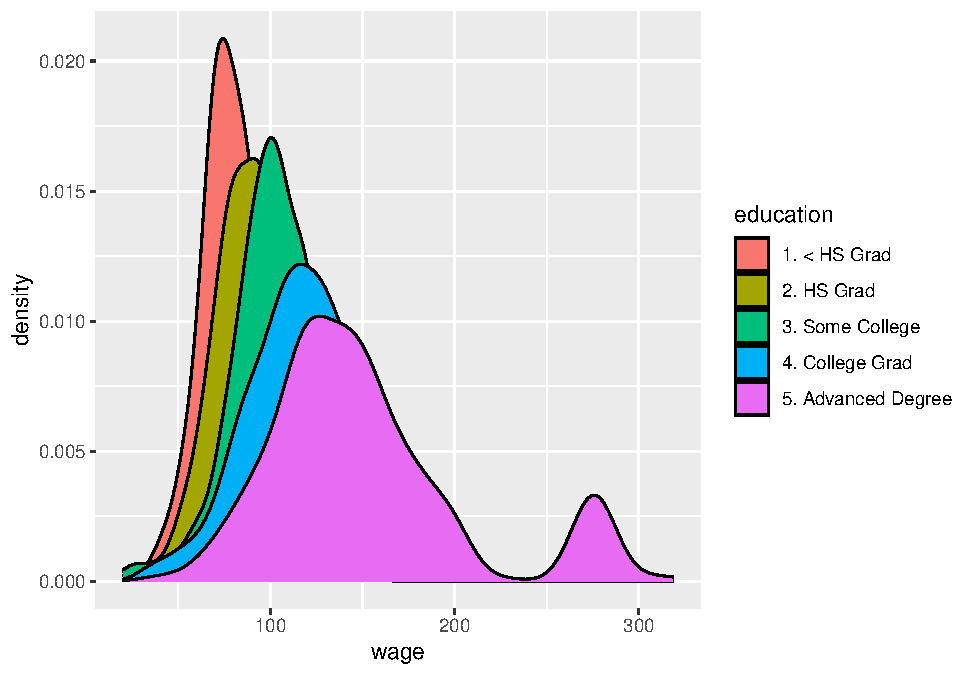
\includegraphics{exploration_files/figure-latex/unnamed-chunk-4-1.pdf}

Make some adjustments:

\begin{Shaded}
\begin{Highlighting}[]
\NormalTok{wage\_df }\SpecialCharTok{\%\textgreater{}\%} 
  \FunctionTok{ggplot}\NormalTok{(}\FunctionTok{aes}\NormalTok{(}\AttributeTok{x =}\NormalTok{ wage, }\AttributeTok{fill =}\NormalTok{ education)) }\SpecialCharTok{+}
  \FunctionTok{geom\_density}\NormalTok{(}\AttributeTok{alpha =} \FloatTok{0.6}\NormalTok{) }\SpecialCharTok{+}
  \FunctionTok{scale\_fill\_brewer}\NormalTok{(}\AttributeTok{palette =} \StringTok{"Blues"}\NormalTok{)}
\end{Highlighting}
\end{Shaded}

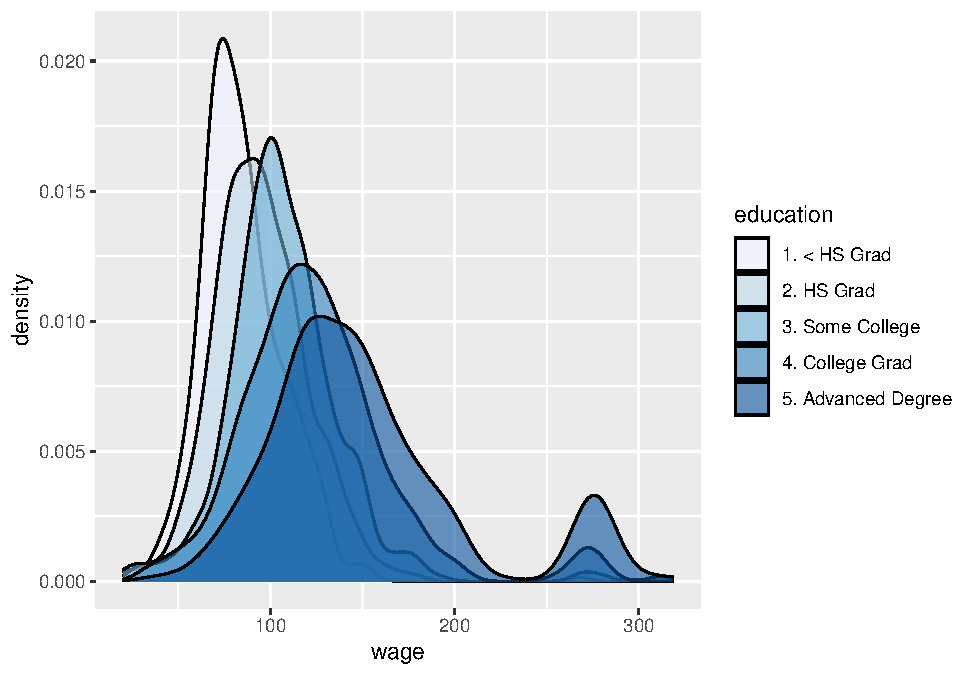
\includegraphics{exploration_files/figure-latex/unnamed-chunk-5-1.pdf}

\hypertarget{boxplot}{%
\chapter{Boxplot}\label{boxplot}}

You should use this method if the data is:

\begin{itemize}
\tightlist
\item
  Categorical (at least ordinal) or
\item
  Numerical
\end{itemize}

In this chapter you will learn how to do some simple data explorations for categorical (ordinal) and numerical variables using boxplots.

\hypertarget{one-variable-3}{%
\section{One variable}\label{one-variable-3}}

\begin{Shaded}
\begin{Highlighting}[]
\NormalTok{wage\_df }\SpecialCharTok{\%\textgreater{}\%} 
  \FunctionTok{ggplot}\NormalTok{(}\FunctionTok{aes}\NormalTok{( }\AttributeTok{x =} \StringTok{""}\NormalTok{, }\AttributeTok{y=}\NormalTok{ wage)) }\SpecialCharTok{+} 
  \FunctionTok{geom\_boxplot}\NormalTok{() }
\end{Highlighting}
\end{Shaded}

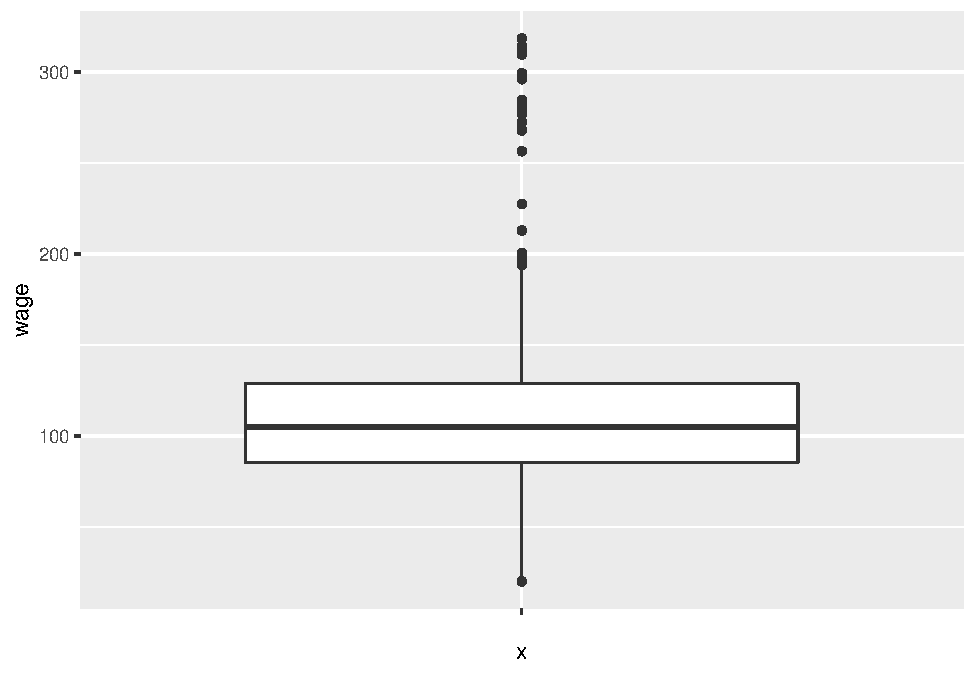
\includegraphics{exploration_files/figure-latex/unnamed-chunk-6-1.pdf}

\hypertarget{two-variables-3}{%
\section{Two variables}\label{two-variables-3}}

\begin{Shaded}
\begin{Highlighting}[]
\NormalTok{wage\_df }\SpecialCharTok{\%\textgreater{}\%} 
  \FunctionTok{ggplot}\NormalTok{(}\FunctionTok{aes}\NormalTok{(}\AttributeTok{x =}\NormalTok{ education, }\AttributeTok{y =}\NormalTok{ wage)) }\SpecialCharTok{+} 
  \FunctionTok{geom\_boxplot}\NormalTok{()}
\end{Highlighting}
\end{Shaded}

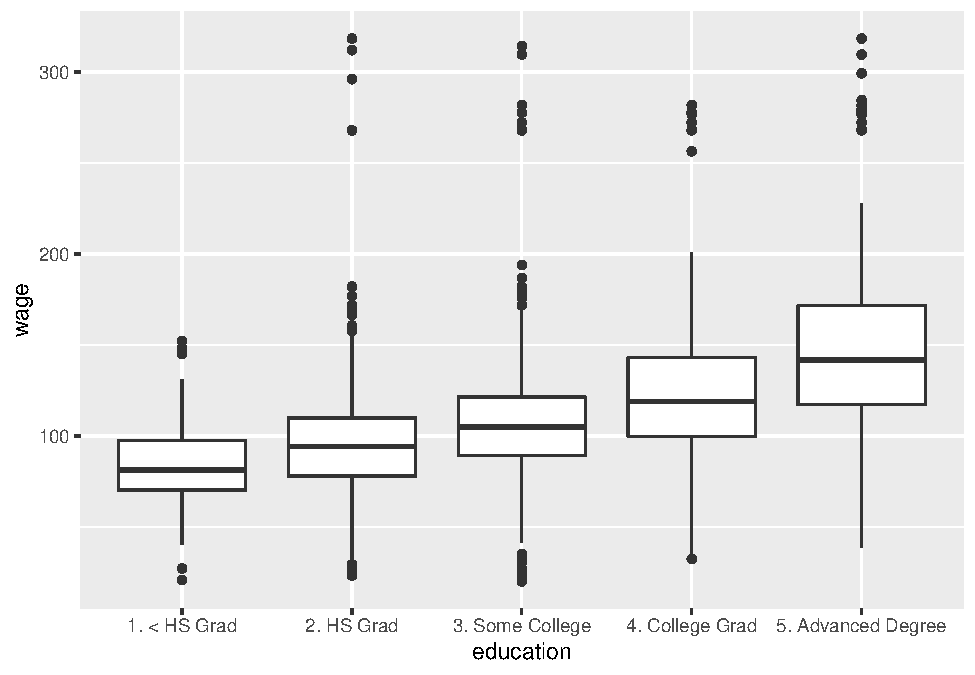
\includegraphics{exploration_files/figure-latex/unnamed-chunk-7-1.pdf}

\hypertarget{scatterplot}{%
\chapter{Scatterplot}\label{scatterplot}}

You should use this method if the data is:

\begin{itemize}
\tightlist
\item
  Numerical
\end{itemize}

\hypertarget{two-numeric-variables}{%
\section{Two numeric variables}\label{two-numeric-variables}}

\begin{Shaded}
\begin{Highlighting}[]
\NormalTok{wage\_df }\SpecialCharTok{\%\textgreater{}\%} 
  \FunctionTok{ggplot}\NormalTok{(}\FunctionTok{aes}\NormalTok{(}\AttributeTok{x =}\NormalTok{ age, }\AttributeTok{y =}\NormalTok{ wage)) }\SpecialCharTok{+}
  \FunctionTok{geom\_point}\NormalTok{()}
\end{Highlighting}
\end{Shaded}

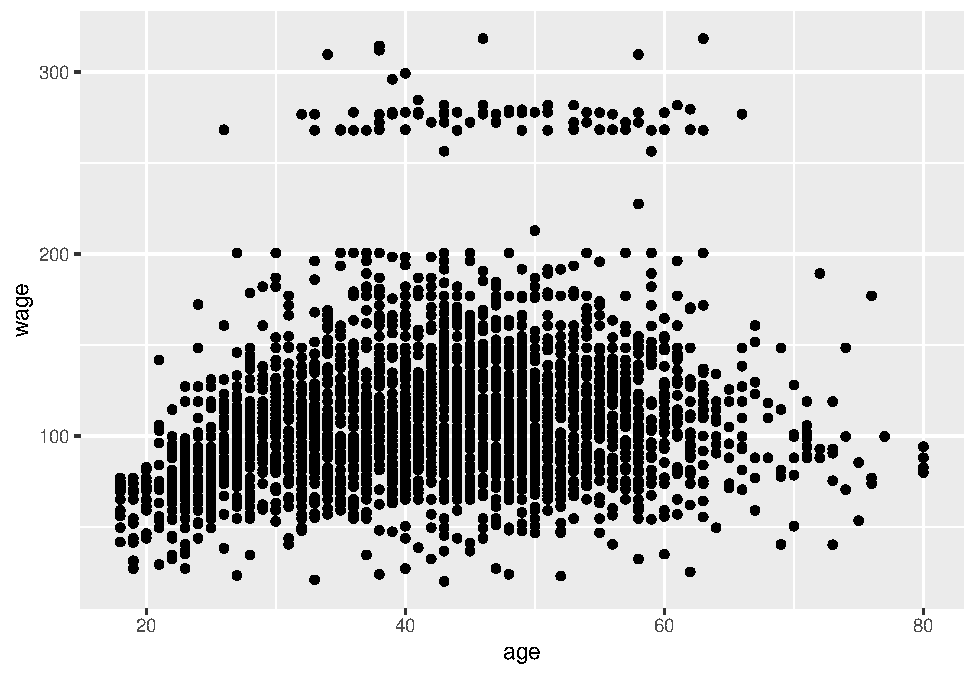
\includegraphics{exploration_files/figure-latex/unnamed-chunk-8-1.pdf}

Use jitter

\begin{Shaded}
\begin{Highlighting}[]
\NormalTok{wage\_df }\SpecialCharTok{\%\textgreater{}\%} 
  \FunctionTok{ggplot}\NormalTok{(}\FunctionTok{aes}\NormalTok{(}\AttributeTok{x =}\NormalTok{ age, }\AttributeTok{y =}\NormalTok{ wage)) }\SpecialCharTok{+}
  \FunctionTok{geom\_jitter}\NormalTok{()}
\end{Highlighting}
\end{Shaded}

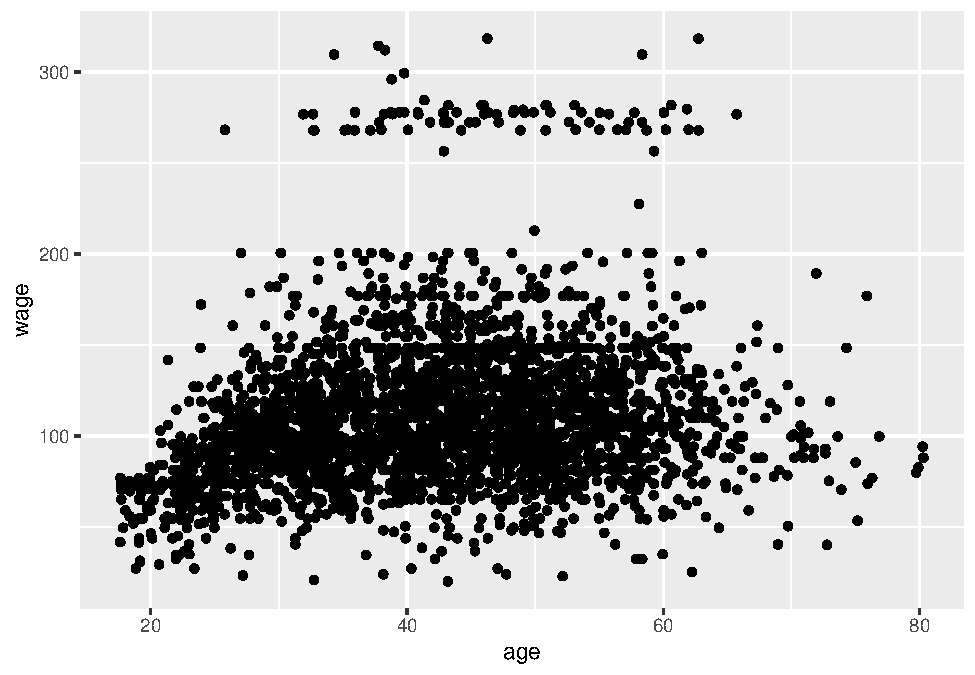
\includegraphics{exploration_files/figure-latex/unnamed-chunk-9-1.pdf}

\hypertarget{two-numeric-one-categorical}{%
\section{Two numeric, one categorical}\label{two-numeric-one-categorical}}

\begin{Shaded}
\begin{Highlighting}[]
\NormalTok{wage\_df }\SpecialCharTok{\%\textgreater{}\%} 
  \FunctionTok{ggplot}\NormalTok{(}\FunctionTok{aes}\NormalTok{(}\AttributeTok{x =}\NormalTok{ age, }\AttributeTok{y =}\NormalTok{ wage, }\AttributeTok{color =}\NormalTok{ jobclass)) }\SpecialCharTok{+}
  \FunctionTok{geom\_jitter}\NormalTok{()}
\end{Highlighting}
\end{Shaded}

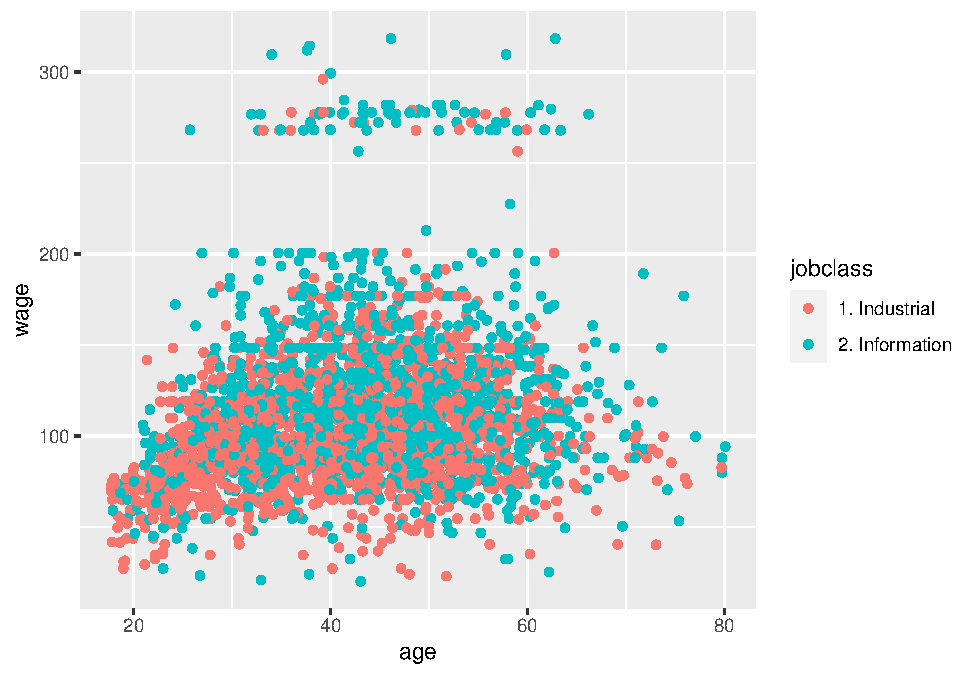
\includegraphics{exploration_files/figure-latex/unnamed-chunk-10-1.pdf}

\hypertarget{line}{%
\chapter{Line graph}\label{line}}

\begin{Shaded}
\begin{Highlighting}[]
\NormalTok{wage\_df }\SpecialCharTok{\%\textgreater{}\%}  
  \FunctionTok{group\_by}\NormalTok{(year) }\SpecialCharTok{\%\textgreater{}\%}  
  \FunctionTok{mutate}\NormalTok{(}\AttributeTok{mean\_wage =} \FunctionTok{mean}\NormalTok{(wage, }\AttributeTok{na.rm =} \ConstantTok{TRUE}\NormalTok{)) }\SpecialCharTok{\%\textgreater{}\%}  
  \FunctionTok{ungroup}\NormalTok{() }\SpecialCharTok{\%\textgreater{}\%} 
  \FunctionTok{ggplot}\NormalTok{(}\FunctionTok{aes}\NormalTok{(}\AttributeTok{x =}\NormalTok{ year, }\AttributeTok{y =}\NormalTok{ mean\_wage)) }\SpecialCharTok{+} 
  \FunctionTok{geom\_line}\NormalTok{() }
\end{Highlighting}
\end{Shaded}

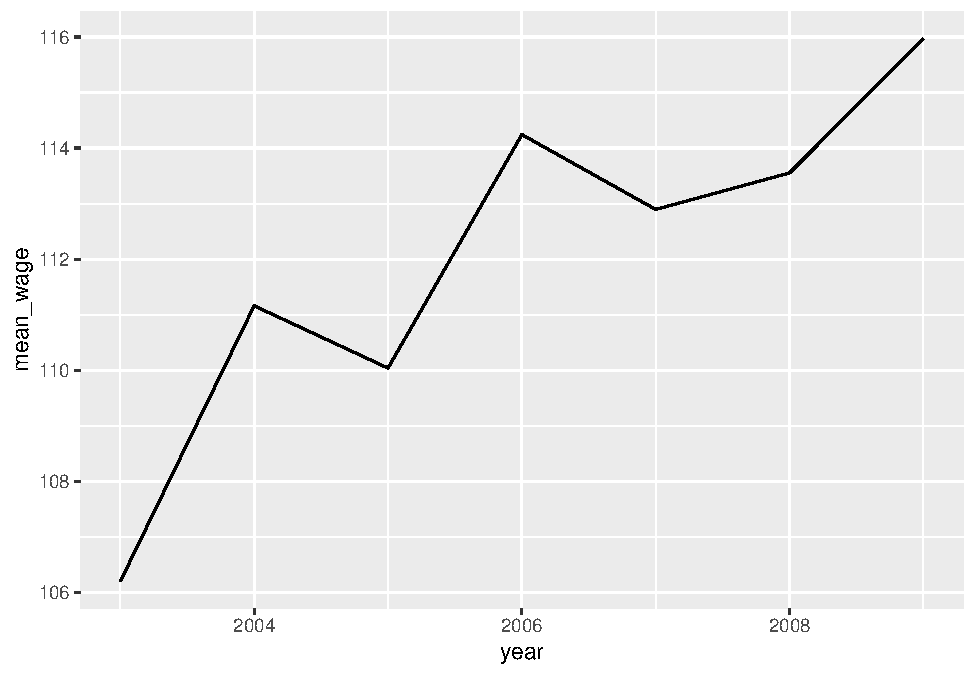
\includegraphics{exploration_files/figure-latex/unnamed-chunk-11-1.pdf}

  \bibliography{book.bib,packages.bib}

\end{document}
